\sectiondate{Les Harkis à Meyrueis}{1963-1965}

\vspace{5mm}

\textbf{Très bref historique}

« Les Harkis : militaires indigènes d’Afrique du Nord qui servaient dans une milice
supplétive (une harka) aux côtés des Français ». Dictionnaire Le nouveau petit Robert 2004

« …restant au contact de leurs familles et attachés à leur territoire, les harkis au
nombre de 30.000 en 1959, ont joué un rôle important comme auxiliaires des troupes
françaises en Algérie de 1954 à 1962 ». Dictionnaire Larousse en 3 vol. 1981

Après la proclamation de l’indépendance de l’Algérie, le 18 Mars 1962, ( Accords
d’Evian ) quelques milliers de harkis purent trouver refuge en France, souvent à
l’initiative d’officiers qui les avaient appréciés mais les autorités françaises interdirent
un rapatriement massif de ces « supplétifs de l’armée française ». La plupart de ceux
qui furent abandonnés et désarmés en Algérie ont été massacrés dans des conditions
abominables.

« … les harkis qui purent se réfugier en France avec leurs familles, après les accords
d’Evian en 1962 furent hébergés dans des camps sommaires, qui devaient rester
transitoires, où tout laissait à désirer : St. Maurice l’Ardoise dans le Gard, Rivesaltes
dans les Pyrénées Orientales, Bias surtout dans le Lot et Garonne et quelques autres.
A la fin de l’année 1962 beaucoup sont évacués dans 75 hameaux forestiers
comprenant plus de 10.000 personnes. L’essentiel est situé dans le Sud-Est de la
France, Languedoc-Roussillon, Provence Côte d’azur et Corse. Entre 10 et 40
travailleurs forestiers selon les hameaux, travaillent pour l’office National des
Forêts. S’occupant de zones rurales, ils constituent souvent des microcosmes à la
périphérie des communes. Ils sont encadrés par un chef de hameau la plupart du temps
un officier des SAS -Section Administrative Spécialisée- et par une monitrice de promotion
sociale ». (Dalila Kerchouche : Destins de Harkis Editions Autrement)

\textbf{Les Harkis à Meyrueis}

Ce sont très exactement 26 familles (131 personnes en tout) qui furent installées dans
des baraquements sur un « bancel » dans la plaine de Ferrussac, au-dessus de la route
à quelques centaines de mètres du village. L’isolement de ce « hameau », comme de
tous les autres, d’ailleurs, est « la formule magique » qui permet de concilier les
intérêts et les préoccupations des services concernés et des communes d’implantation.
Ils constitueront pour un bon nombre de rapatriés musulmans un véritable « filtre »
qui leur permettra, dans un stade transitoire, et grâce à l’encadrement (…) de
s’adapter progressivement…

\textbf{Les enfants :} Il y eut de 21 naissances à « la Foulatière » ou à l’hôpital de Florac, au
cours des années 1963, 1964 et 1965. Les parents donnent à tous les enfants (deux
exceptés) un prénom français suivi d’un prénom arabe. On peut supposer une forte
pression des responsables du hameau., en vue d’une « assimilation » plus rapide de
leurs enfants.

Les enfants étaient donc scolarisés à Meyrueis dans deux préfabriqués dans la cour de
l’école communale : deux classes mixtes sans doute puisque la mixité avait été
instaurée en 1942 ou 1943 à la retraite de Mme. Chalmeton.
Mais trois filles, les aînées, probablement allaient à l’école des Sœurs, qui elle, n’était
pas mixte.
Il y eut des décès parmi les enfants, à Meyrueis comme à Villemagne ou ailleurs.

Ainsi à Meyrueis, est enregistré le décès de Simone Zaara née le 27 Février 1965 et
morte le 3 mars. Le chef du hameau souligne dans son rapport mensuel qu’il y a eu
problème, il s’exprime de la façon suivante :à Meyrueis il y a deux cimetières, le
cimetière Chrétien et le cimetière des Protestants ou ensevelir Simone ?
Ce sera dans le cimetière protestant. Mais en 2006 je n’ai pas trouvé trace de sa
tombe.

A Villemagne le « hameau forestier » avait été installé dans le « village
Nègre ». Baraquements des mines de la Pennaroya, totalement isolé, à plusieurs km de
Camprieu, le seul village avoisinant. Un garçon est enterré là, dans le petit cimetière
près de l’Eglise (désaffectée).

A St. Etienne de Valdonnez, pour l’ensevelissement d’un enfant le maire refusa
l’accès du cimetière et l’enfant fut enterré en pleine forêt.
Sans commentaire !!!

\textbf{Contacts avec la population :}

Ils furent minimes :

Pour les fêtes de Noël 1964, Françoise et Josiane Ribot étaient venues de Nîmes, pour
« conter Noël avec talent » dit le rapport du responsable. Le maire M. Védrines était
présent et des cadeaux furent distribuées.
Lors d’une fête de Noël en 1965, avec 37 enfants, le curé, accompagné de l’abbé,
était monté au hameau mais les sœurs n’avaient pu venir à cause de la neige et du
mauvais temps.
Le pasteur M. Bertrand prit une fois la défense d’un harki qui n’avait pas reçu des
indemnités auquel il avait droit. Mais il n’était pas passé par la voie hiérarchique ce
qu’on lui fait remarquer, cependant avec amabilité !
A Noël 1965, une chorale protestante de Nîmes avait organisé une grande fête pour
les harkis de Villemagne, à Camprieu, avec chants bien sûr, cadeaux, gâteaux...

\textbf{A noter :}

\begin{itemize}
    \item Une antenne avait été installée en Décembre 1964, pour un poste de télévision.
    Mais on ne sait pas si le poste a été installé....
    
    \item Les enfants de Harkis étaient partis en colonie de vacances à Agde dans le
    Centre de Batipaume, fondé par Robert Fages, (\textit{voir plus loin : Meyrueisiens
    connus...})
    
    \item \textit{« Nous avons toujours ressenti une grande défiance à notre égard, et même un certain mépris
    dans les villages mais tout autant à Mende et pourtant nos pères ont combattu pour la
    France »} nous dit S. un . de ces fils de harki.
\end{itemize}

\section{Réactions du Conseil Municipal}

« Ce hameau forestier » c’est l’appellation officielle, avait été édifié, comme les 74
autres hameaux dans des conditions très sommaires, écrit Michel Roux dans son livre
« Les harkis, les oubliés de l’histoire 1954-1991 » P.312 – La Découverte- La qualité médiocre
des matériaux de construction, la précarité, l’insalubrité et l’exiguïté des logements,
les défauts de viabilisation sont le lot de la quasi-totalité de ces regroupements
théoriquement conçus pour s’effacer rapidement de la carte...

A Meyrueis, à Truscas (Hérault) et Mirande (Gers) – comme disent Abi Slimane et Finas
dans le livre -Regroupement et dispersion-) le chauffage est insuffisant et l’humidité pénètre
partout. Avec leur défaut d’isolation les logements sont travaillés de l’intérieur, par
en dessous comme par en dessus ? par une pourriture insistante qui les ronge à un
rythme accéléré. Le chauffage ? quand il parvient (mais à un prix exorbitant) à
réchauffer les habitants, génère une sorte de brouillard, une vapeur « tropicale-
humide » : micro-climat du micro-monde forestier ; le hameau est le cocon morbide
du Français-Musulman ».

Leur séjour à Meyrueis ne laissa que peu de traces dans les archives municipales. Il
faut dire que ces hameaux forestiers ou camps de harkis relevaient directement du
Ministère des Rapatriés et du Ministère de l’Agriculture dont dépend le Service des
Eaux et Forêts. Les communes n’avaient pas leur mot à dire, les ministères
s’entendant directement avec les Eaux et Forêts où beaucoup seront employés. J’ai
noté seulement deux paragraphes dans les délibérations du Conseil Municipal de
Meyrueis :

\begin{quote}
« Le 11 Décembre 1962, le conseil municipal est appelé à donner son avis sur le
transport des élèves de familles harkies qui doivent être installées dans la commune.
Le conseil municipal donne un avis favorable pour le ramassage de ces élèves sous
réserve que cette opération n’occasionne aucun frais pour la commune ».
\end{quote}

Un peu plus tard le 30 Juillet 1963 :

\begin{quote}
« L’implantation d’un camp de Harkis à Roquedols, soit 131 personnes, porte la
population de Meyrueis de 1198 à 1329 habitants ; cette augmentation se traduit,
pour la commune, par des charges nouvelles : admission à l’Assistance médicale,
alimentation, eau potable etc. Pour ces raisons le Conseil estime juste que ces
habitants soient ajoutés à la population légale de la commune avec toutes les
conséquences de droit. »
\end{quote}

\begin{quote}
« Les municipalités, en général, - note toujours Michel Roux (op. cité) - manifestent
d’entrée une réticence non dissimulée à l’implantation de ces Algériens sur leur
territoire communal. Cependant l’éloignement des hameaux et leur encadrement
paramilitaire les rassurent. En outre, à l’assurance de n’avoir pas à subir les charges
imputables à l’arrivée d’une population importante, s’ajoute la promesse qu’elle sera
employée à des travaux d’aménagement dans les territoires communaux. Enfin
nombre de hameaux sont considérés comme temporaires... »
\end{quote}

\subsection{Leur vie à Ferrussac}

Jean et Thérèse Gaillard-Arnal de l’Oultre, à Pont Vieux, me donnèrent bien des
précisions sur l’installation de ces familles harkies. En Lozère, 160 familles environ
furent installées dans ce qu’on a appelé des « hameaux forestiers » : 52 à Villefort, 26
à Chadenet, 26 à Cassagnas-Haut, 26 à Culture, et enfin 26 à Meyrueis au lieu-dit La
Foulatière, un long « bancel », à 200m en amont de la chaussée de Roquedols au -
dessus de la route de Ferrussac, limité par le vallon de Roquedoulet.

Jean Gaillard, menuisier, vint à Meyrueis avec les camions apportant les baraques
préfabriquées et prêtes à être montées. C’est une entreprise de Saint-Pardoux-la-
Rivière en Dordogne, spécialisées dans la fabrication de villas, salles de classe,
baraques de chantier préfabriquées, qui obtint le marché.
Les familles harkies furent donc installées à Meyrueis le 15 mars 1963 dans ces
baraquements légers pour hébergement provisoire

\begin{quote}
\textit{« C’était, me dit-Jean Gaillard, des baraques légères à parois de bois isolées par
seulement 5cm de laine de verre ( nous sommes en 1963 ). Les familles disposaient de
2 ou 3 pièces suivant leur composition : une ou deux femmes -l’épouse et la
concubine- Chaque logement avait une cuisine avec évier et une cheminée. Il y avait
donc, en tout, 60 à 70 adultes accompagnés par le même nombre d’enfants : les
baraques se chauffaient rapidement mais se refroidissaient instantanément dès que le
feu « tombait », et l’été, par grand soleil il fallait arroser les toits pour faire baisser
la chaleur étouffante à l’intérieur.. Les toilettes étaient à l’extérieur. A côté des
logements une baraque servait de foyer où les hommes pouvaient se réunir après le
travail. Le soubassement subsiste encore »}
\end{quote}

Quant à Thérèse Gaillard, Melle. Arnal à l’époque, elle avait pendant sa scolarité, à la
fin des années 50, été très présente auprès d’une grand mère âgée et malade, l’aidant
pour les repas, la toilette etc. Elle venait d’obtenir un brevet d’aide-ménagère-
comptable. Elle fut embauchée pour travailler auprès des femmes harkies, d’abord
dans un hameau perdu au-dessus de Villefort, le Pouget, afin de faciliter leur
adaptation.

\begin{quote}
\textit{« J’ai posé ma candidature pour Meyrueis quand j’ai su qu’on allait implanter un
hameau près de Ferrussac. Elle a été retenue en partie parce que je disposais d’une
2cv indispensable pour les trajets. J’étais désormais « Monitrice d’Action Sociale ».
Lorsque la 2cv arrivait, toutes les femmes se disaient l’une à l’autre « C’est la
sociale ! ».
Une de mes plus grosses difficultés fut d’obtenir l’ouverture des fenêtres et des volets
pour aérer et laisser entrer le soleil et la lumière. Il y avait aussi les soins pour les
bébés : les femmes les emmaillotaient totalement, la tête seule dépassait, et les
nourrissons ne pouvaient bouger ni bras ni jambes. Car il y eut des naissances . Ce
ne fut pas une mince affaire d’emmener les femmes, avec leurs maris bien sûr, à la
maternité de Florac ou de Mende. Il fallait également leur apprendre à acheter aux
épiciers ambulants, des aliments et des légumes différents de ceux d’Algérie,
proposés sur place par Caiffa, « Pissou » de Florac, Rigal etc. Mme. Richard de
Ferrussac les voyait fréquemment en leur apportant le lait de ses vaches.
Il fallut leur apprendre à consulter le médecin ou à l’appeler, heureusement le Dr.
Juliette Cabanel était bien acceptée car c’était une femme. »}
\end{quote}

\begin{center}
    {\Large\bfseries Les Harkis à Meyrueis}
    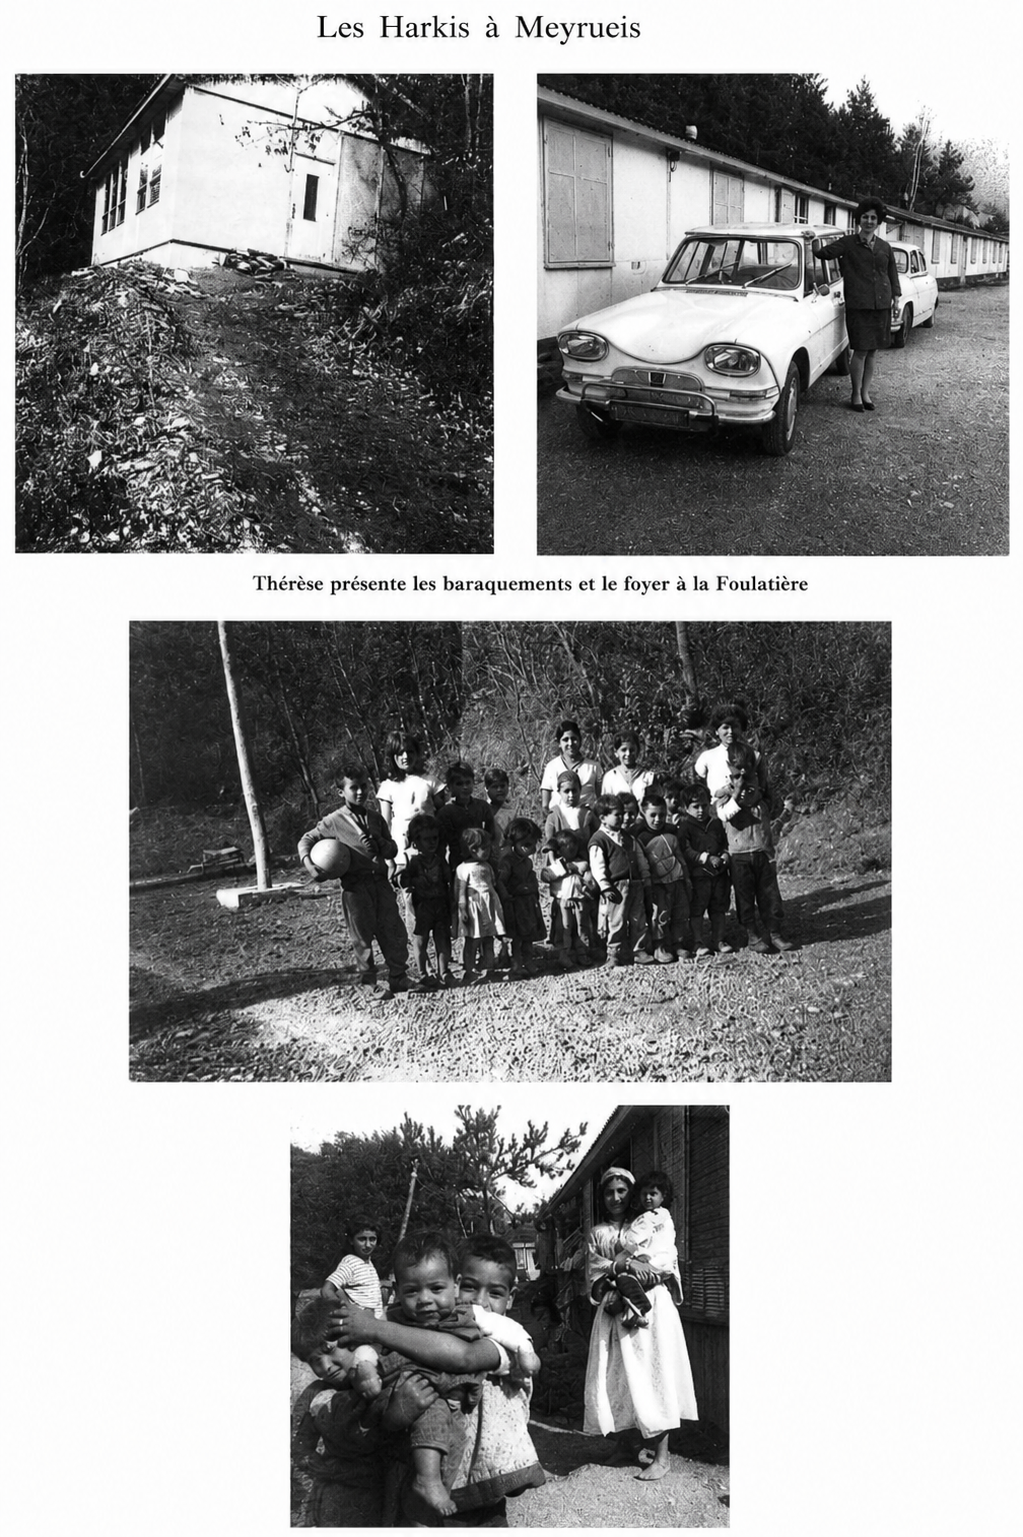
\includegraphics[width=\textwidth]{imgs/124}
\end{center}

Elles me demandèrent de leur apprendre à tricoter : elles s’installaient autour de
moi, toujours pieds nus et assises sur leur talons, jamais sur des chaises. Elles étaient
fort habiles et confectionnaient par exemple de petites corbeilles tissées avec de la
laine pour y placer galettes et gâteaux au miel...

Le responsable du hameau, Pedro, était un ancien adjudant d’Algérie, parlant arabe,
qui organisait les chantiers pour les hommes et veillait à la bonne entente dans le
camp. Lui succédèrent Susini puis Normand. Quant aux enfants, deux classes, en
préfabriqué, avaient été construites dans la cour de l’ancienne école de Meyrueis :
elles ont subsisté jusqu’aux années 2000 ! Un ramassage scolaire avait été mis en
place et c’est René Fages -- Fafa -- (il avait été caché au Moulin d’Ayres après avoir été blessé
lors des combats de la Parade, 20 ans auparavant), qui faisait office de chauffeur.
A notre égard ils furent tous d’une gentillesse extrême, avec de multiples attentions,
de petits cadeaux et des bols de couscous suffisants pour une famille (très)
nombreuse ! ».

A Ferrussac, Mme. Richard-Valdeyron et son mari, me donne quelques précisions
complémentaires :

\begin{quote}
\textit{« Je leur apportais, peut-être une vingtaine de litres de lait mais ce n’était pas tous
les jours. Mon mari laissait le bidon au bord de la route mais c’est moi qui devais
l’apporter aux femmes ; souvent elles le laissaient au soleil, attendant qu’il caille en
devenant aigre.}

\textit{Certains avaient plusieurs femmes Il y en avait un qui en avait même trois C’était le
plus âgé, le caïd. Sa première femme, la plus âgée, avait tout le pouvoir, les deux
autres, bien plus jeunes, obéissaient. C’est lui qui faisait la circoncision pour les
garçons. Parfois le médecin (le Dr. Rouzier) venait vérifier, à cause de l’hygiène.}

\textit{C’était de bons clients pour les commerçants car ils payaient rubis sur l’ongle.. Si
l’appoint manquait, nul besoin de le demander le lendemain. Parfois les hommes
descendaient à Meyrueis ; ils allaient au café et, de temps à autre, c’est le taxi de
Combemale qui les ramenait, lorsqu’ils avaient trop bu. Il conduisait également, à
l’hôpital ceux qui étaient gravement malades. »}
\end{quote}

\section*{Les Harkis au travail}

Les harkis étaient employés par les \og Eaux et Forêts \fg{}. Ils formaient deux équipes :
La 1\textsuperscript{ère}. travaillait à la pépinière de Roquedols sous la direction de M. Boulet, la 2\textsuperscript{ème}
était affectée aux travaux en forêt : elle élargit la route empierrée entre le Villaret et
Rousses. Pour ce faire, elle démolit et fit disparaître les restes de l’ancien moulin de
Rousses à 100m en aval du hameau et aussi l’ancien porche de la maison Martin, (nos
cousins Martin de Ferrussac et Raffègues. La maison et la propriété Martin avaient été vendues vers
1960 aux Eaux et Forêts), par lequel passait le chemin. Trop étroit il empêchait le passage
des camionnettes ou camions pour le transport du bois.
Les harkis, continuèrent jusqu’à la Pépinière, et tracèrent la route forestière
jusqu’au col de la Caumette permettant une sortie directe de la vallée du Béthuzon vers
l’Aigoual.

Surtout, on les mettait souvent à contribution pour donner un coup de main aux
pompiers en cas de feux des forêts et, bien sûr, ils exploitaient la forêt pour le compte
de l’Administration. Leur salaire était minime.
Lorsque les hameaux furent supprimés en 1965, plusieurs familles furent envoyées à
Lodève dans des logements HLM, d’autres à Mende dans un foyer Sonacotra, d’autres
en Provence.

A la fin Novembre 2006 j’ai pu glaner d’autres renseignements sur les Harkis de
Meyrueis et de Lozère auprès des deux Inspecteurs des Eaux et Forêts, successivement
en poste à Mende à cette époque : M. Paul Cabane et M. Marcel Gavalda..

C’est à \textbf{M. Cabane} qu’échut la responsabilité, dans les derniers mois de
1962, d’installer les harkis et leurs familles, parfois très nombreuses dans des
implantations choisies par la Direction des Eaux et Forêts en Lozère, dans le Gard ou
en Provence, à Meyrueis en ce qui nous concerne..

\begin{quote}
\textit{« Le grand problème fut de les loger, me dit-il, et les baraques ou les cabanes
étaient très légères. Ce ne devait être que des logements provisoires pour quelques
mois en attendant des installations définitives : en fait ils restèrent bien plus
longtemps. Seuls furent assez vite supprimés les hameaux qui étaient en altitude à
l’ombre et au froid.}

\textit{Lors de leur arrivée il n’y eut pas de problème pour leur installation. Et au début,
tout cela fut assez positif. Mais des agents d’encadrement ou des hommes de
l’extérieur, chevilles de syndicats les « chauffèrent de plus en plus » Ils travaillèrent
de moins en moins sur les chantiers forestiers, les pistes d’exploitation, les vacations
avec les pompiers, et ils en demandèrent de plus en plus. Et bien sûr on ne pouvait
approcher les mères ni leurs enfants »}
\end{quote}

\textbf{M. Gavalda} arrive à Mende en 1967. Donc trois ans après la mise en place des
hameaux forestiers.

\begin{quote}
\textit{« Je garde un souvenir ému des premiers contacts que j’eus avec eux. Je venais de
passer 15 ans au milieu des berbères du Haut Atlas au Maroc. Je connaissais
quelques mots de berbère et j’eus grand plaisir à retrouver une majorité de kabyles
auprès desquels je n’hésitais pas à revêtir djellaba ou gandoura.}

\textit{Il appartenait au service des Eaux et Forêts de choisir les chantiers, de définir les
travaux, les plantations, l’ouverture ou l’entretien de pistes forestières. Je disposais
d’une ligne budgétaire très encadrée pour les salaires, le matériel...}

\textit{Mais surtout ils devinrent « fantassins du feu », auxiliaires des pompiers, qui ne
disposaient que de bien peu de matériel : les camions modernes bien équipés
n’existaient pas, ni, à plus forte raison, les hélicoptères bombardiers d’eau ou les
Canadairs.}

\textit{Les harkis avaient seulement des pelles, des pioches, des battes pour frapper le feu
ou des haches pour faire des coupe-feux ou des contre-feux, et les incendies dans le
massif de l’Aigoual étaient fréquents et violents. A cette époque on n’avait pas
encore inventé les « tours de guet » et on ne pouvait surveiller les départs de feu
comme on peut le faire aujourd’hui avec les petits avions d’observation.}
\end{quote}

\textit{Le service forestier a essayé de faciliter leur vie dans ces petites communautés où la
vie n’était pas toujours drôle..}

\textit{Finalement c’est en 1965, après 3 ans de séjour à Meyrueis, qu’ils furent relogés
dans des appartements plus modernes et mieux équipés à Mende (Sonacotra) et à
Lodève.
Il y eut même un projet, beaucoup plus tard, en 1980, de tous les regrouper en
Provence, puis de les transférer - une idée de technocrates parisiens du Ministère
de l’Agriculture - en Haute Corse dans une des zones les plus isolées et difficile
d’accès. Il n’y eut qu’un cri : pas question. Le service forestier comme le préfet
prirent position en leur faveur. Et rien ne se passa. Malgré toutes les vicissitudes
qu’ils connurent, leur état d’esprit m’apparaissait assez serein.}

\textit{Et maintenant ? 25 ans plus tard ?}

\textit{A Mende plusieurs familles se sont installées définitivement et ont fait souche. Les
rapports avec la population locale n’ont pas posé de gros problèmes ; il y a un
Conseiller municipal, des sportifs, (foot, coureurs ...) Au début le taux de chômage
était élevé mais petit à petit des employeurs locaux en ont embauché, la majorité
d’entre eux se sont casés ou ont même lancé de petites affaires.
Les harkis d’origine étaient assimilés à des employés de l’ONF avec droit à la
retraite. Ils ont demandé que leurs fils disposent du même statut mais ce leur fut
refusé par crainte de « ghettoisation. »}

\begin{center}
\textbf{En guise de conclusion provisoire}
\end{center}

Aux dires des témoins, il semble que, même s’il n’y eut pas beaucoup de contacts
avec la population de Meyrueis - mais on sortait tout juste de la guerre d’Algérie- les
choses se passèrent moins mal, dans ces petits « hameaux », que dans les grands
camps comme Bias en Lot et Garonne, Saint Maurice l’Ardoise dans le Gard ou
Rivesaltes dans l’Aude, où furent hébergées des centaines de familles de harkis avec
une discipline de fer, des barbelés et des portails fermés la nuit, des prénoms français
donnés d’autorité par les chefs de camp aux bébés venant de naître etc...
Malheureusement je n’ai pu, à ce jour, retrouver d’anciens harkis de la Foulatière ni
leurs femmes ni leurs enfants...

\begin{flushright}
\textit{A Meyrueis\\
Le 26 Novembre 2006}
\end{flushright}

Avant de rassembler et photocopier ces documents le 10 Décembre 2006, j’ai pu jeter
un coup d’œil sur des rapports de responsables du hameau de Meyrueis. J’en ignorais
l’existence jusqu’alors ! j’ai pu, également, avoir les coordonnées d’un fils de harki
de Villemagne, installé à Mende, mais pas encore celles de familles ayant séjourné à
Meyrueis. Voici cependant quelques renseignements complémentaires : notés dans ces
rapports ou d’après la très brève conversation téléphonique avec M. S, fils de harki.



